\documentclass[a4paper,11pt,landscape,twocolumn]{article}

\usepackage{préambule}
\usepackage{clipboard}
\usetikzlibrary{arrows.meta}

\makeatletter
\renewcommand{\maketitle}{%
{\scriptsize colle dans ton cahier d'exercices}
	\begin{center}
		\LARGE
		\uline{\@title}
		\vspace{0.5em}
	\end{center}
}
\makeatother

\title{Activité : Chasse au trésor}
\date{}
\author{}

\begin{document}

\Copy{Trésor}{
	\maketitle

	\begin{exercice}\
		\begin{center}
			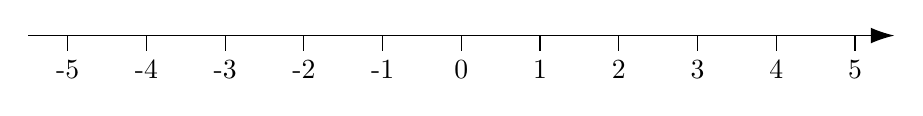
\begin{tikzpicture}
				\draw[-{Latex[length=3mm, width=2mm]}] (-5.5,0) -- (5.5,0);

				\foreach \x in {-5,...,5} {
						\draw (\x,0) -- ++(0,-0.2) node[below] {\x};
					}
			\end{tikzpicture}
		\end{center}

		\begin{itemize}
			\item Place un point \textbf{A} au point d'abscisse 3.
			\item Place \textbf{B} le symétrique de A par rapport au point d'abscisse 0. Quelle est l'abscisse du point obtenu ? .......
			\item Place \textbf{C} le symétrique de B par rapport au point d'abscisse $-1$. Quelle est l'abscisse du point obtenu ? .......
		\end{itemize}
	\end{exercice}

	\begin{exercice}\

		Un trésor est enterré le long d'une ligne de train proche de la gare de Lyon ! Pour le trouver, on dispose des instructions suivantes :

		\begin{itemize}
			\item Démarre 5{,}5 kilomètres avant la gare de Lyon.
			\item 1 kilomètre avant la gare, il y a un poste électrique : déplace toi jusqu'au symétrique de ton point actuel par rapport à ce poste.
			\item Éloigne-toi de 2{,}5 kilomètres de la gare.
			\item Fait en sorte de diviser la distance entre la gare et toi par 4.
			\item Tourne-toi vers la gare, et avance de 2{,}7 kilomètres.
		\end{itemize}

		Dessine une \textbf{droite graduée} représentant la ligne de train, en plaçant la gare de Lyon au point d'abscisse $0$.

		Ensuite, suit les instructions pour déterminer la position du trésor !\vspace{1em}

		\begin{center}
			\large
			\begin{tabular}{lll}
				Le trésor est ..... kilomètres & avant & la gare. \\
				                               & après &
			\end{tabular}
		\end{center}
	\end{exercice}
}

\newpage

\setcounter{exercice}{0}

\Paste{Trésor}


\end{document}